\documentclass[12pt]{article}
\usepackage{geometry}
\geometry{a4paper}
\usepackage{amsmath}
\usepackage{graphicx}
\usepackage{hyperref}
\usepackage[numbers]{natbib}
\usepackage{tikz}
\usepackage{booktabs}
\setlength{\emergencystretch}{1em}

\title{Comparative Analysis of Shake-Shake Regularization in a ResNet-Like Architecture for CIFAR-10 Image Classification}
\author{Liam Cawley}
\date{Course project; technical corrections, October 2026}

\begin{document}

\maketitle

\begin{abstract}
This note describes the regularization methods considered in a CIFAR-10 course project and records the accuracies reported in the original project report. The comparison includes changes in network depth as well as Cutout, Mixup, and Shake-Shake. It does not isolate a general ranking of these methods. This revision corrects the residual-gradient formula, ResNet layer counting, and the distinction between ordinary residual connections and the parallel branches required by Shake-Shake.
\end{abstract}

\section{Introduction}
The CIFAR-10 dataset, comprising 60,000 32x32 color images across 10 classes, is selected for its balance between complexity and manageability, making it an ideal candidate for evaluating image classification algorithms. This dataset allows for a meaningful comparison without the need for extensive computational resources. Central to this study is Shake-Shake regularization, a technique that introduces randomness in the network's forward and backward passes to reduce overfitting and improve generalization.

The dataset's moderate complexity and size facilitate rapid experimentation while still presenting challenges representative of real-world scenarios. This study extends a basic Convolutional Neural Network (CNN) model, enhancing its performance through advanced regularization techniques and architectural modifications.

\subsection{Basic CNN Model}
A Convolutional Neural Network (CNN) is a deep learning algorithm which can take in an input image, assign learnable weights and biases to various aspects/objects in the image and be able to differentiate one from the other.
The foundational model is a CNN composed of convolutional layers, batch normalization, dropout, and dense layers, structured to process the CIFAR-10 dataset effectively. The network architecture is designed to learn hierarchical feature representations from the input images.

\subsection{Mathematical Formulation}
The core operations in a CNN are convolution, pooling, and fully connected layers.

\subsubsection{Convolution Layer}
In a convolution layer, a convolution operation is applied to the input data with the use of a filter or kernel to produce a feature map. This operation is defined as:
\begin{equation}
    F_{ij} = \sum_{m}\sum_{n}I_{(i+m)(j+n)}K_{mn}
\end{equation}
where \( F \) is the feature map, \( I \) is the input image, and \( K \) is the kernel.

\subsubsection{Pooling Layer}
Pooling (subsampling or down-sampling) reduces the dimensionality of each feature map but retains the most important information. Average pooling and max pooling are common types.

\subsubsection{Fully Connected Layer}
The fully connected layer takes the output of the previous layers and turns them into a single vector, which can be an input for the next stage, such as a softmax layer for classification.

\subsubsection{Activation Function}
An activation function like ReLU (Rectified Linear Unit) is used to introduce non-linear properties to the network.
\begin{equation}
    f(x) = max(0, x)
\end{equation}

\pagebreak

\begin{figure}[h!]
\centering
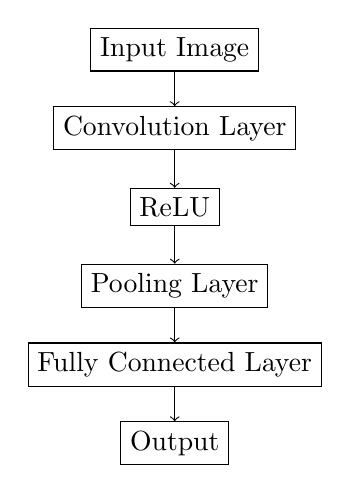
\begin{tikzpicture}
\node (input) [draw, rectangle] {Input Image};
\node (conv1) [draw, rectangle, below of=input] {Convolution Layer};
\node (relu1) [draw, rectangle, below of=conv1] {ReLU};
\node (pool1) [draw, rectangle, below of=relu1] {Pooling Layer};
\node (fc) [draw, rectangle, below of=pool1] {Fully Connected Layer};
\node (output) [draw, rectangle, below of=fc] {Output};

\draw [->] (input) -- (conv1);
\draw [->] (conv1) -- (relu1);
\draw [->] (relu1) -- (pool1);
\draw [->] (pool1) -- (fc);
\draw [->] (fc) -- (output);
\end{tikzpicture}
\caption{Architecture of a Convolutional Neural Network}
\end{figure}

\subsection{ResNet50 Architecture}
The conventional ResNet-50 depth counts 49 convolutional layers on the main path and one final fully connected layer. Pooling layers are excluded from that count. Its residual connections provide a direct path for activations and gradients. For an identity shortcut, a residual block has the form:
\begin{equation}
    \text{output} = \mathcal{F}(\text{input}, \{W_i\}) + \text{input}
\end{equation}
where \(\mathcal{F}\) is the residual function (e.g., a stack of two convolution layers), \(\{W_i\}\) are the weights, and input is the input feature map.

\subsection{Residual Learning}
The key innovation in ResNet is the introduction of a so-called “skip connection” that bypasses one or more layers. 

\subsubsection{Identity Mapping}
Identity mapping in ResNet is a crucial component that facilitates the training of very deep networks. In the simplest form, the identity mapping is realized by skip connections that bypass one or more layers.

\paragraph{Mathematical Perspective of Identity Mapping}
The identity mapping in ResNet can be defined as a connection that skips one or more layers and performs an element-wise addition operation with the output of the stacked layers. Mathematically, this can be represented as:
\begin{equation}
    \text{output} = \mathcal{F}(x, \{W_i\}) + x
\end{equation}
where \(x\) is the input to the block, and \(\mathcal{F}\) is the function representing the stacked layers. 

This approach alleviates the vanishing gradient problem by allowing gradients to flow directly through the skip connections during backpropagation. It effectively allows the layers to learn residual functions concerning the layer inputs, thus easing the training of deeper networks.

\paragraph{Proof of Concept}
To demonstrate the effectiveness of identity mapping, consider the gradient flow during backpropagation. The gradient of the loss function with respect to the input \(x\) can be computed as:
\begin{equation}
    \nabla_x \mathcal{L} =
    \left(I + J_{\mathcal{F}}(x)\right)^\top \nabla_{\text{output}}\mathcal{L}
\end{equation}
where gradients are column vectors and \(J_{\mathcal{F}}\) is the Jacobian of the residual branch. The identity matrix \(I\) accounts for the shortcut.

The shortcut supplies an additive gradient term; it does not guarantee that the total gradient is nonzero. For example, \(J_{\mathcal{F}}=-I\) cancels it.


\begin{figure}[h!]
\centering
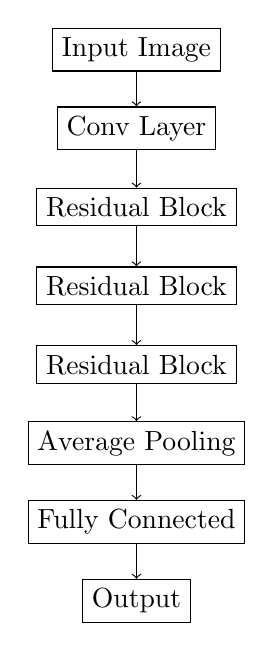
\begin{tikzpicture}
\node (input) [draw, rectangle] {Input Image};
\node (conv1) [draw, rectangle, below of=input] {Conv Layer};
\node (res1) [draw, rectangle, below of=conv1] {Residual Block};
\node (res2) [draw, rectangle, below of=res1] {Residual Block};
\node (res3) [draw, rectangle, below of=res2] {Residual Block};
\node (avgpool) [draw, rectangle, below of=res3] {Average Pooling};
\node (fc) [draw, rectangle, below of=avgpool] {Fully Connected};
\node (output) [draw, rectangle, below of=fc] {Output};

\draw [->] (input) -- (conv1);
\draw [->] (conv1) -- (res1);
\draw [->] (res1) -- (res2);
\draw [->] (res2) -- (res3);
\draw [->] (res3) -- (avgpool);
\draw [->] (avgpool) -- (fc);
\draw [->] (fc) -- (output);
\end{tikzpicture}
\caption{Schematic of a residual network; each box can contain multiple layers.}
\end{figure}


\subsection{Advanced Regularization Techniques}
The project uses two established data augmentation methods, Cutout and Mixup. Their effects depend on the training setup; neither guarantees generalization.

\subsubsection{Cutout}
Cutout, a form of data augmentation, involves randomly removing square regions from the input images during training. Mathematically, it can be represented as:
\begin{equation}
  \text{Cutout}(I) = I \odot M
\end{equation}
where \(I\) is the input image, and \(M\) is a binary mask with a square region set to 0.

\subsubsection{Mixup}
Mixup creates new training examples by linearly combining pairs of images and their labels. It is expressed as:
\begin{equation}
  \text{Mixup}(I_1, I_2, y_1, y_2, \lambda) = (\lambda I_1 + (1 - \lambda) I_2, \lambda y_1 + (1 - \lambda) y_2)
\end{equation}
where \(I_1, I_2\) are images, \(y_1, y_2\) are their respective labels, and \(\lambda\) is a mixing coefficient.

\subsection{Shake-Shake Regularization}
Shake-Shake requires a modified block with two parallel residual branches
\cite{gastaldi2017shake}. In the common two-branch formulation, the training
forward pass is
\[
 y=x+\alpha F_1(x)+(1-\alpha)F_2(x),
\]
where \(\alpha\) is sampled during training. The backward pass uses a separately
sampled coefficient \(\beta\):
\[
 \nabla_x\mathcal{L}
 =\left(I+\beta J_{F_1}(x)+(1-\beta)J_{F_2}(x)\right)^\top\nabla_y\mathcal{L}.
\]
Using different coefficients requires a custom backward rule or an equivalent
stop-gradient construction; ordinary differentiation of the forward expression
would reuse \(\alpha\). At evaluation, the residual branches are averaged with
weights \(1/2\). An ordinary single-branch ResNet block does not already contain
these two residual branches.

\section{Experimental Design and Evaluation}
The experimental setup involves training the modified CNN models with Cutout, Mixup, and Shake-Shake regularization on the CIFAR-10 dataset. The performance of each model is evaluated based on accuracy, precision, recall, and F1 score. Preprocessing in this study involves normalizing image pixel values to a range between 0 and 1, ensuring consistent scaling across the dataset and stabilizing the training process. Convolutional layers automatically learn relevant features from the image data, allowing the model to identify and utilize complex patterns without manual feature extraction.

\subsection{Data Preprocessing and Feature Selection}
Prior to training, the CIFAR-10 images are normalized, and data augmentation techniques are applied. Feature selection is inherent in the convolutional layers of the CNN, which are designed to automatically learn relevant features from the data.

\subsection{Performance Metrics}
The primary performance metric is classification accuracy. However, precision, recall, and F1 score provide a more nuanced understanding of the model's performance, especially in handling class imbalances.

\subsection{Challenges and Solutions}
Implementing advanced regularization techniques like Shake-Shake and Mixup presents challenges, particularly in ensuring model stability and preventing overfitting. Regular monitoring and hyperparameter tuning are essential to address these issues.

\subsection{Limitations and Future Work}
The original report gives one metric value per configuration, without repeated-seed uncertainty. It includes no small-data sweep, GradCAM study, or experiment combining all three regularizers.

\subsection{Design Choices and Parameter Tuning}
The choice of hyperparameters, such as the size of the cutout mask and the value of \(\lambda\) in Mixup, is critical. Extensive experimentation is required to determine the optimal values for these parameters.


\section{Reported results and their scope}

The following values are transcribed from Table 1 of the original project
report. They have not been regenerated from retained checkpoints.

\begin{center}
\begin{tabular}{lr}
\toprule
Configuration & Reported accuracy (\%)\\
\midrule
Three-layer CNN & 78\\
Ten-layer CNN & 85\\
Ten-layer CNN with Cutout & 87\\
Ten-layer CNN with Mixup & 88\\
Custom ResNet-50 & 92\\
Custom ResNet-50 with Shake-Shake & 93\\
\bottomrule
\end{tabular}
\end{center}

The 78-to-88 comparison includes a depth change and Mixup. It cannot be
attributed to combined regularization. The ResNet comparison reports a
one-percentage-point difference. Because the methods were applied to different
architectures, these results do not establish which regularizer is best under
matched conditions. An attribution study would hold architecture, optimizer,
training schedule, and data split fixed and repeat training across seeds.

\section{Conclusion}
The reported configurations improved over their respective baselines in this
course exercise. Their individual mechanisms and general superiority were not
established by the comparison. The technical definitions above describe how the
methods operate and the controls a more complete comparison would need.

\begin{thebibliography}{9}
\bibitem{gastaldi2017shake}
Xavier Gastaldi. \emph{Shake-Shake Regularization}.
2017. \url{https://arxiv.org/abs/1705.07485}.
\bibitem{he2016resnet}
Kaiming He et al. \emph{Deep Residual Learning for Image Recognition}.
CVPR, 2016. \url{https://arxiv.org/abs/1512.03385}.
\bibitem{zhang2018mixup}
Hongyi Zhang et al. \emph{mixup: Beyond Empirical Risk Minimization}.
ICLR, 2018. \url{https://arxiv.org/abs/1710.09412}.
\bibitem{devries2017cutout}
Terrance DeVries and Graham W. Taylor.
\emph{Improved Regularization of Convolutional Neural Networks with Cutout}.
2017. \url{https://arxiv.org/abs/1708.04552}.
\end{thebibliography}

\end{document}
